\documentclass[12pt,a4paper]{article}

\usepackage[utf8]{inputenc}
\usepackage[T2A]{fontenc}
\usepackage[russian]{babel}
\usepackage{amsmath, amssymb, amsthm, amsfonts}
\usepackage{graphicx}
\usepackage{hyperref}
\usepackage[margin=2cm]{geometry}
\usepackage{cite}
\usepackage{setspace}
\onehalfspacing

\hypersetup{
    pdftitle={Исследование влияния вида задачи для уравнения гармонического осциллятора на решение PINN},
    pdfauthor={Донецков А.Д., Бакакин В.Д.},
    pdfsubject={Отчет},
    pdfkeywords={PINN, ОДУ, гармонический осциллятор, машинное обучение}
}

\title{Исследование влияния вида задачи для уравнения гармонического осциллятора на решение PINN}
\author{
Донецков А.Д.\thanks{E-mail: andrey.donetskov@gmail.com},
Бакакин В.Д.,
Жулев Е.М. \\
\textit{НИЯУ МИФИ}
}
\date{\today}

\begin{document}

\maketitle

\begin{abstract}
В данном отчёте рассматривается применение метода физически -- информированных нейронных сетей \textbf{PINN} (Physics-Informed Neural Networks) для решения уравнения гармонического осциллятора с вынуждающей силой. Исследуется влияние различных формулировок задачи Коши на точность и сходимость метода PINN. Представлены сравнительные результаты, демонстрирующие различия в скорости сходимости, устойчивости обучения и точности.
\end{abstract}

\section{Введение}
Одной из важных задач в области вычислительной физики и механики является решение уравнений движения гармонического осциллятора. Классический гармонический осциллятор описывается различными дифференциальными уравнениями как второго, так и первого порядка. В последнее десятилетие активно развиваются нейросетевые методы решения дифференциальных уравнений, в частности метод физически-информированных нейронных сетей (PINN) \cite{Lagaris1998,Raissi2019}.

Цель данного исследования --- сравнить влияние различных формулировок задачи Коши для уравнения гармонического осциллятора на точность и эффективность метода PINN.

\section{Постановка задачи}
Рассматриваются три различных формулировки задачи Коши для уравнения гармонического осциллятора с вынуждающей силой, по 2 набора параметров для каждой - для случаев резонанса и его отсутствия:

\subsection{ОДУ второго порядка}
Уравнение вида
\begin{equation}
\begin{cases}
\dfrac{d^2x}{dt^2} + \omega_0^2 x = -A\cos(\omega t), \\
x(0) = x_0, \\
\dfrac{dx}{dt}(0) = v_0.
\end{cases}
\end{equation}
непосредственно описывает динамику гармонического осциллятора.

\textbf{Применение:}
\begin{itemize}
    \item \textbf{Физика колебаний:} Моделирование механических систем, таких как пружинные маятники или электрические колебательные контуры, где присутствуют гармонические колебания.
    \item \textbf{Анализ устойчивости:} Исследование устойчивости систем, подверженных периодическим внешним воздействиям.
\end{itemize}

\subsection{Системы ОДУ первого порядка}
\begin{equation}
\begin{cases}
\dfrac{dx}{dt} = y, \\
\dfrac{dy}{dt} = -\omega_0^2 x - A\cos(\omega t), \\
x(0) = x_0, \\
y(0) = v_0.
\end{cases}
\end{equation}

\begin{equation}
\begin{cases}
\dfrac{dx}{dt} = \omega_0 y - \dfrac{A}{\omega}\sin(\omega t), \\
\dfrac{dy}{dt} = -\omega_0 x, \\
x(0) = x_0, \\
y(0) = \dfrac{v_0}{\omega_0}.
\end{cases}
\end{equation}

\textbf{Применение:}
\begin{itemize}
    \item \textbf{Численные методы:} Многие численные алгоритмы, такие как методы Рунге -- Кутты, разработаны для систем первого порядка, что делает эту форму удобной для компьютерного моделирования.
    \item \textbf{Сложные системы:} Анализ систем с несколькими степенями свободы, где каждая степень описывается своим уравнением первого порядка.
\end{itemize}

\textbf{Примечание:}
Разные системы дифференциальных уравнений первого порядка могут быть полезны в случаях, когда форма упрощает аналитическое или численное решение, в зависимости от характера внешней силы или других факторов.

\section{Ключевые особенности PINN}

\begin{minipage}[t]{0.45\textwidth}
    \small
    \textbf{Преимущества PINN:}
    \begin{itemize}
        \item Интеграция физических законов в процесс обучения для получения физически корректных решений.
        \item Использование автоматического дифференцирования для эффективного вычисления градиентов сложных выражений.
        \item Применимость к различным задачам, включая ОДУ, УЧП и их системы.
    \end{itemize}
\end{minipage}
\hfill
\vrule width 0.5pt
\hfill
\begin{minipage}[t]{0.45\textwidth}
    \small
    \textbf{Ограничения PINN:}
    \begin{itemize}
        \item Трудности с аппроксимацией разрывных функций.
        \item Низкая эффективность при решении жестких и хаотических систем ОДУ.
        \item Застревание в локальных оптимумах.
        \item Сложности в балансировке различных компонентов функции потерь.
    \end{itemize}
\end{minipage}

\section{Методология}

Для сравнительного анализа во всех 3 случаях использовалась одинаковая конфигурация нейросети: 1 входной нейрон принимает время, 5 промежуточных слоёв по 20 нейронов, один или два выходных нейрона в зависимости от системы. 
Функцией активации был выбран синус.
Нейрость обучалась на временном отрезке $[-5, 15]$ с делением в $0.05$.
Для решения задачи использовался метод PINN. Основная идея PINN состоит в обучении нейронной сети, которая аппроксимирует решение дифференциального уравнения.
Функционал потерь $loss = loss_{interior} + \lambda_{bc} * loss_{boundary}$ состоит из двух частей:
\begin{enumerate}
    \item Потери на уравнении (MSE по residual), учитывающие форму дифференциального уравнения.
    \item Потери на граничных условиях (MSE между предсказанием и истинным значением).
\end{enumerate}
Весовой коэффициент ограничения ($\lambda_{bc}$) выл выбран 50.
Обучение модели проводилось с использованием оптимизатора, такого как Adam с шагом обучения $10^{-3}$, для минимизации функции потерь. Этот оптимизатор показывает себя наиболее эффективно для PINN.

\newpage
\section{Результаты}
Для каждой системы было произведено пять результатов обучения. Для случая с резонансом и без него. В качестве метрики использовалось \textbf{MAE} (mean absolute error) между аналитическим и полученным решением. В ходе экспериментов было получено следующее:
\begin{itemize}

    \item \textbf{Система ОДУ второго порядка(1):} Обеспечивает высокую точность и быструю сходимость, хотя часто теряет локальные минимумы во время обучения. См. рисунки~\ref{fig:loss_second_order}~\ref{fig:loss_second_order_resonance}.

    \begin{figure}[h!]
        \centering
        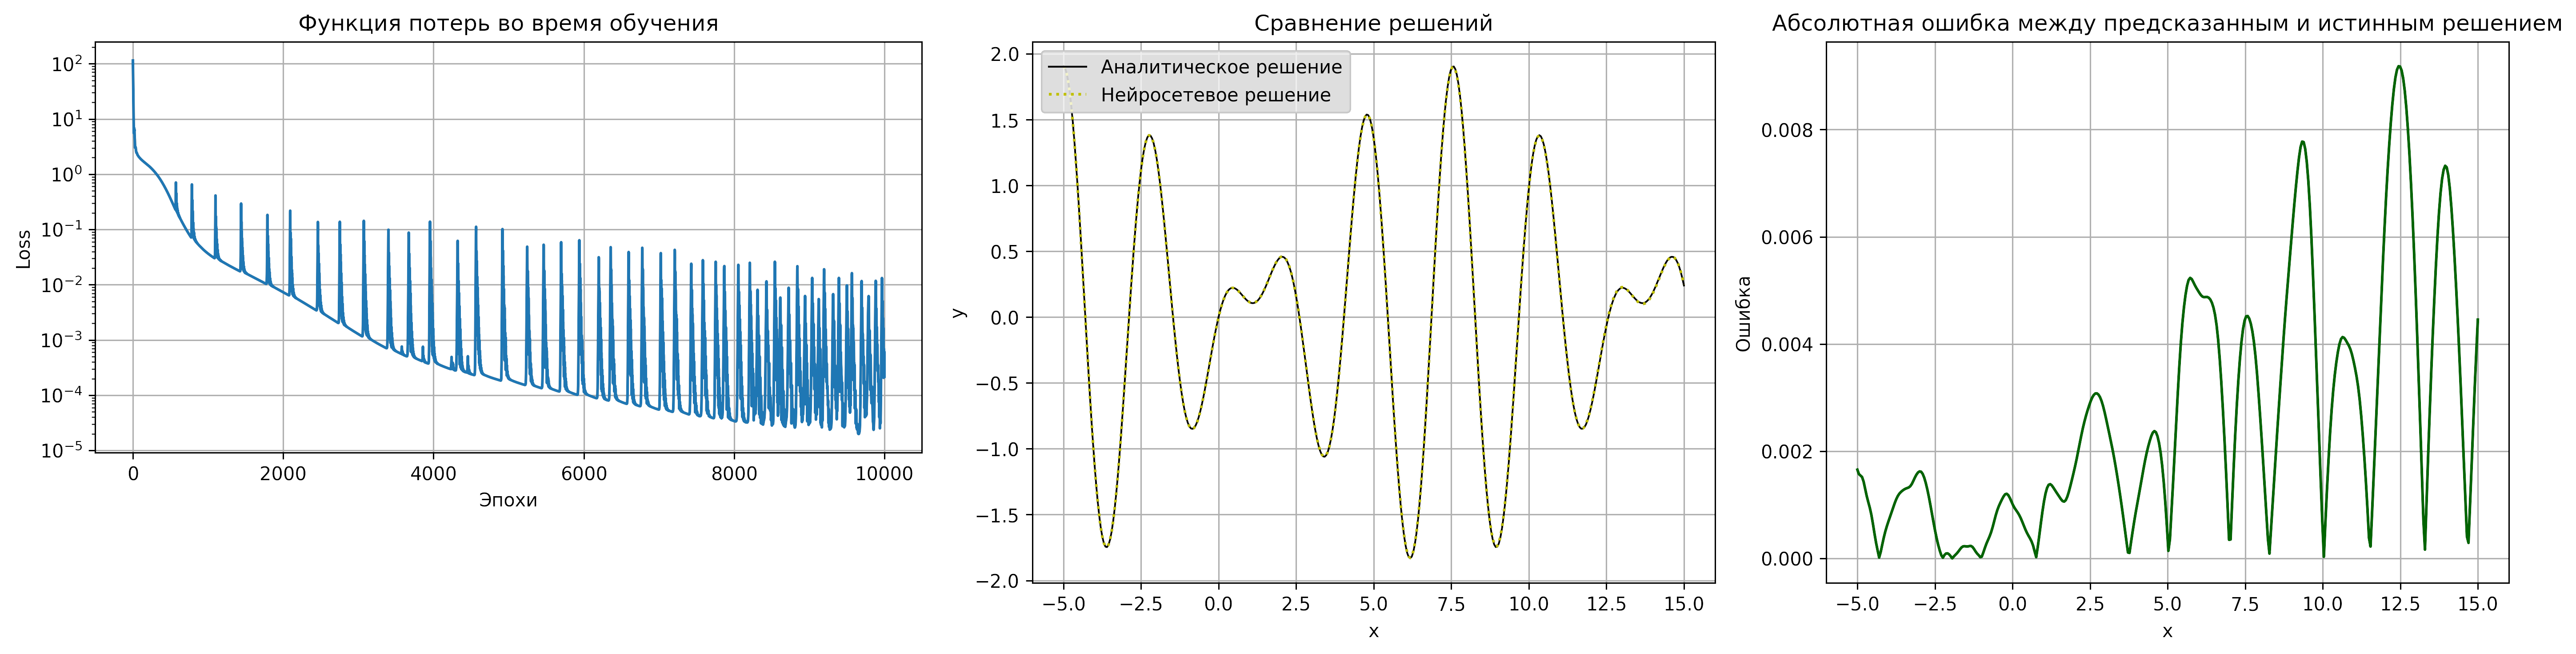
\includegraphics[width=1\textwidth]{images/Loss&x_ODE_of_the_second_order.png}
        \caption{Функция потерь для ОДУ второго порядка}
        \label{fig:loss_second_order}
    \end{figure}

    \begin{figure}[h!]
        \centering
        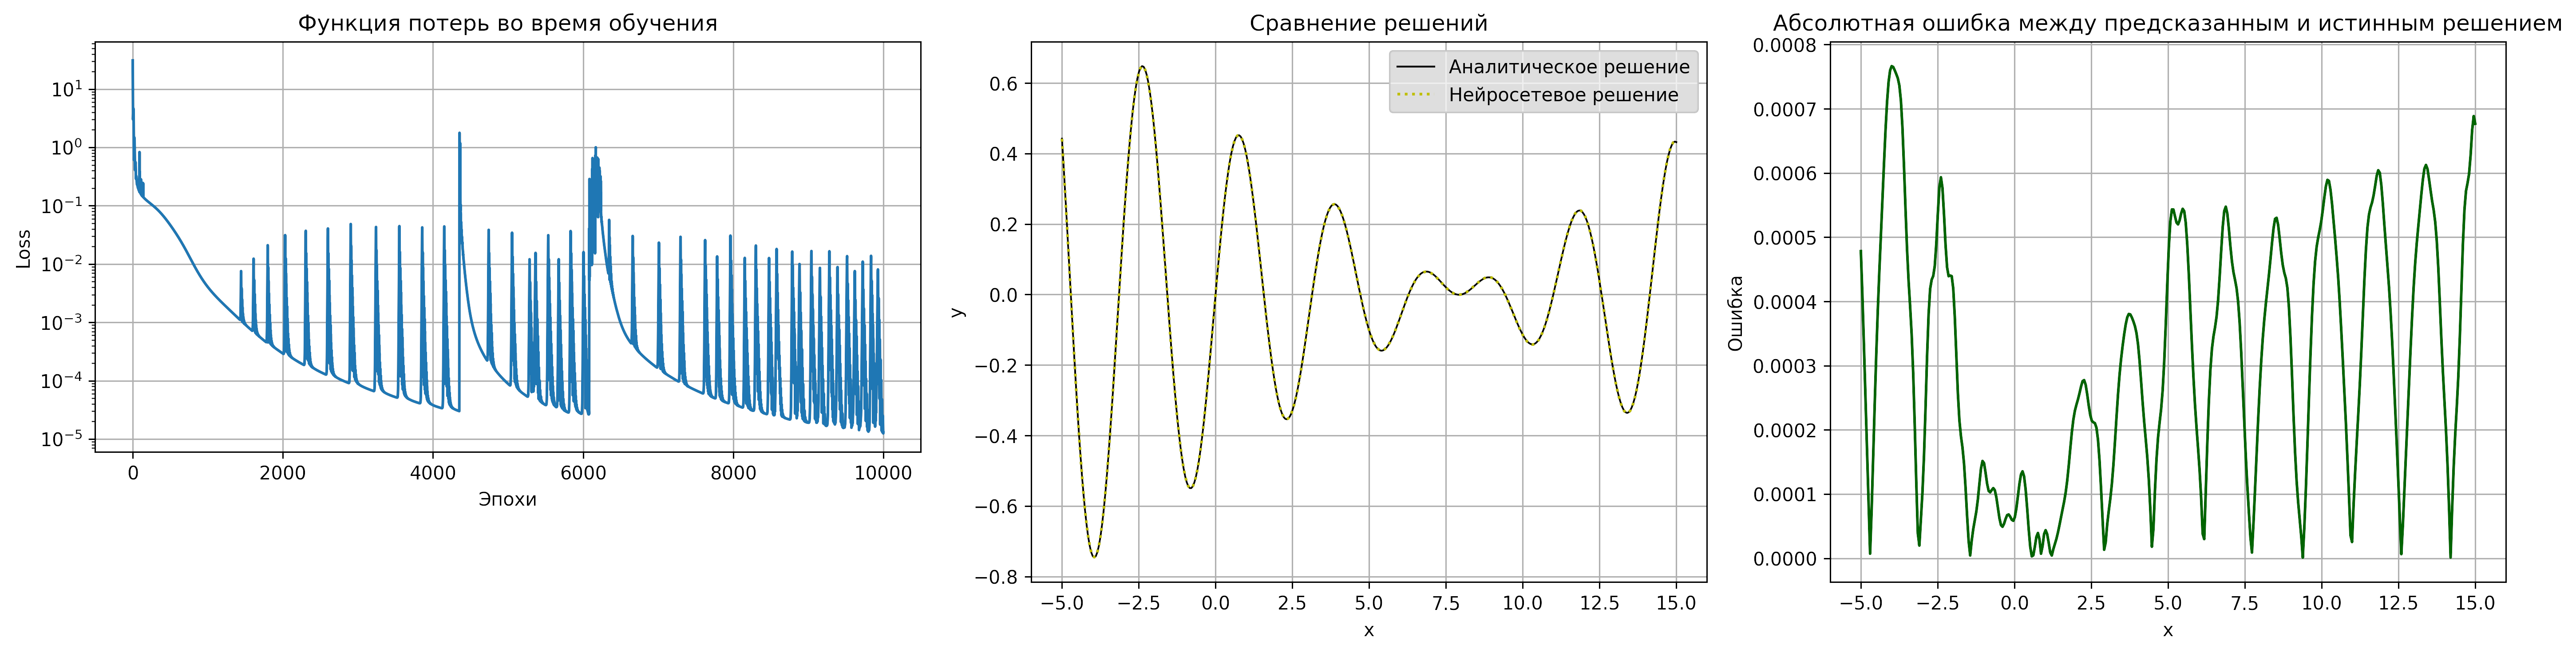
\includegraphics[width=1\textwidth]{images/Loss&x_ODE_of_the_second_order_resonance.png}
        \caption{Функция потерь для ОДУ второго порядка с резонансом}
        \label{fig:loss_second_order_resonance}
    \end{figure}

    \begin{table}[h!]
        \centering
        \begin{tabular}{|c|c|}
        \hline
        \textbf{MAE $x, 10^{-2}$} & \textbf{MAE $\dfrac{dx}{dt}, 10^{-2}$} \\
        \hline
        1,1879 & 2,4357 \\
        1,2033 & 2,4247 \\
        1,6343 & 3,0803 \\
        1,2127 & 2,4514 \\
        1,1406 & 2,3287 \\
        \hline
        \end{tabular}
        \caption{ОДУ второго порядка без резонанся}
    \end{table}

    После 5 замеров средняя MAE как $x$, так и $\dfrac{dx}{dt}$ меньше, чем у ОДУ первого порядка.

    \newpage
    \item \textbf{Система ОДУ первого порядка(2):} Демонстрирует более стабильный, но медленный процесс обучения и менее точные результаты. См. рисунки~\ref{fig:loss_first_order}~\ref{fig:loss_first_order_resonance}.
    
    \begin{figure}[h!]
        \centering
        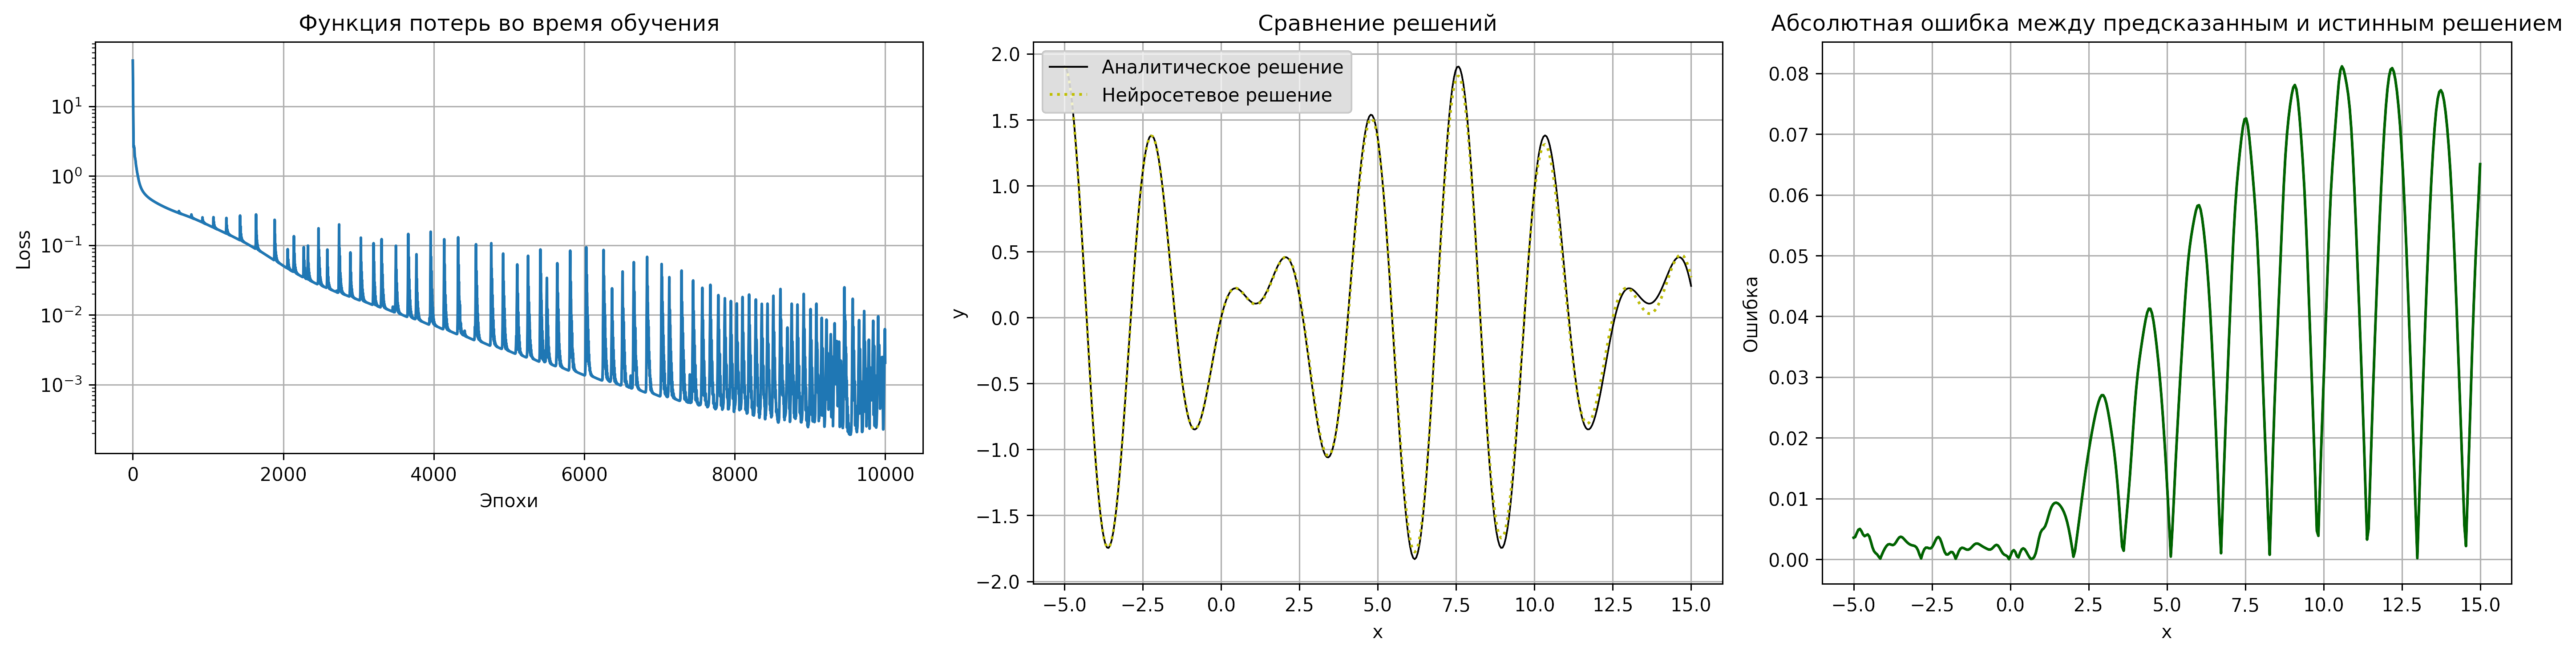
\includegraphics[width=1\textwidth]{images/Loss&x_ODE_of_the_first_order.png}
        \caption{Функция потерь для системы ОДУ первого порядка}
        \label{fig:loss_first_order}
    \end{figure}

    \begin{figure}[h!]
        \centering
        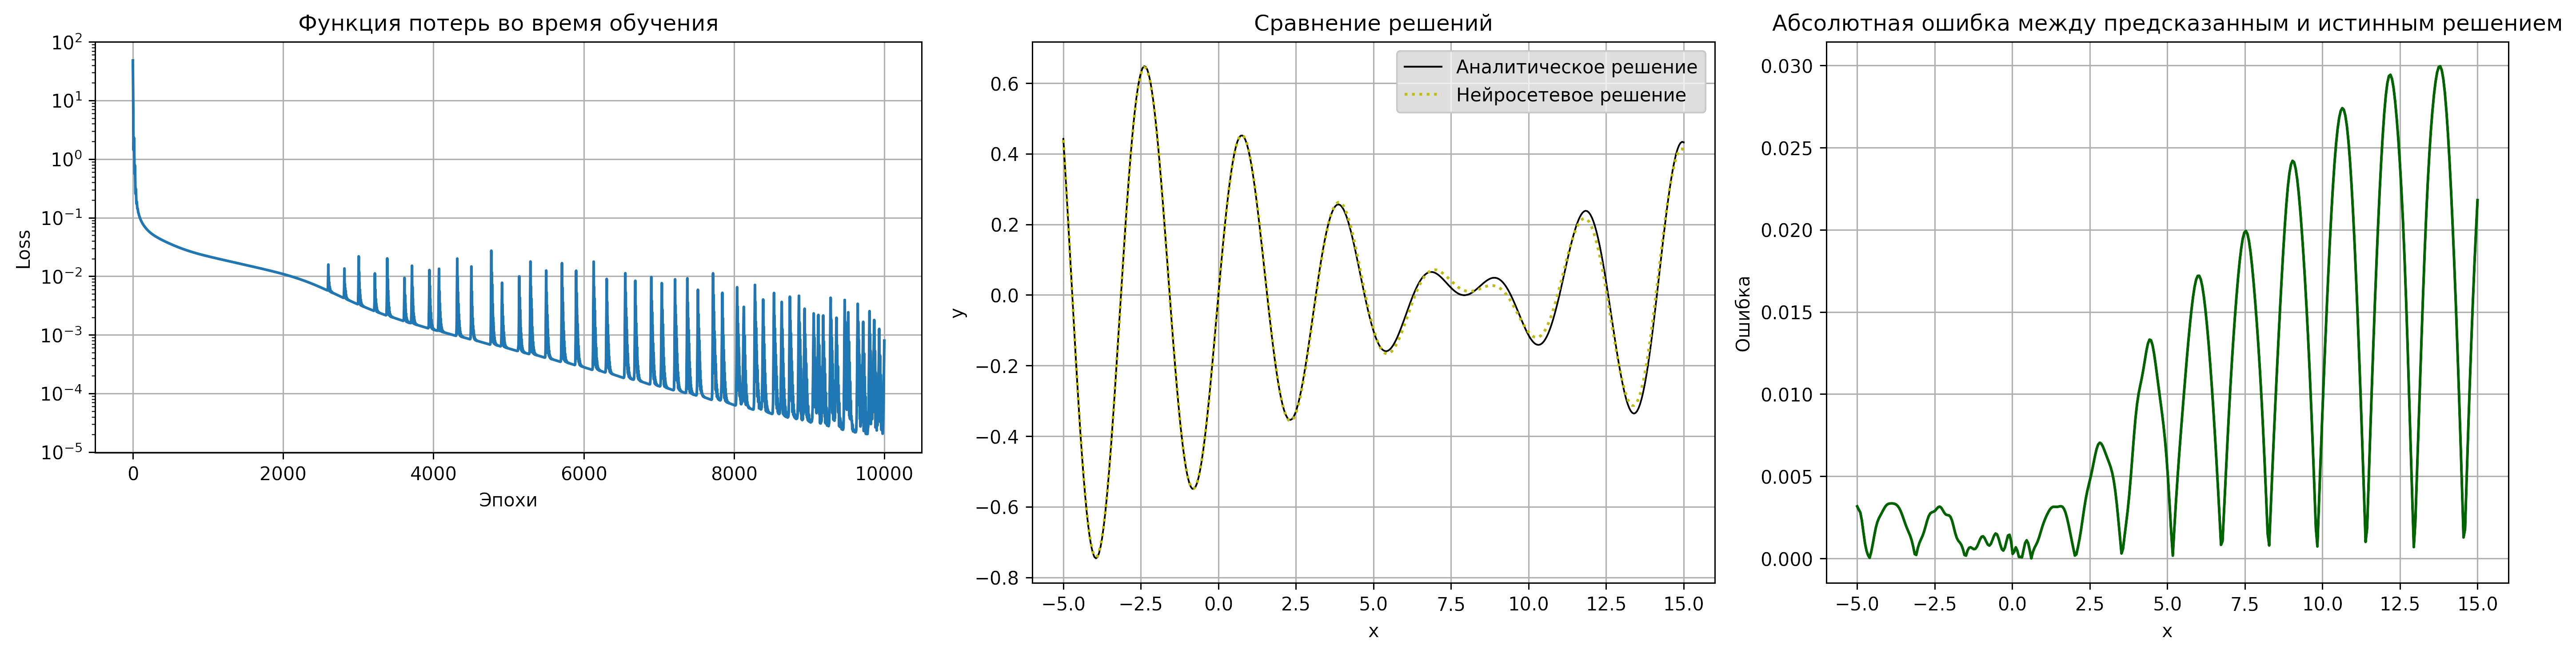
\includegraphics[width=1\textwidth]{images/Loss&x_ODE_of_the_first_order_resonance.png}
        \caption{Функция потерь для системы ОДУ первого порядка с резонансом}
        \label{fig:loss_first_order_resonance}
    \end{figure}

    \begin{table}[h!]
        \centering
        \begin{tabular}{|c|c|}
        \hline
        \textbf{MAE $x, 10^{-2}$} & \textbf{MAE $y, 10^{-2}$} \\
        \hline
        4,8092 & 9,8869 \\
        3,5429 & 7,2853 \\
        3,6680 & 7,4666 \\
        3,6264 & 7,4309 \\
        2,5681 & 5,4567 \\
        \hline
        \end{tabular}
        \caption{ОДУ первого порядка без резонанся}
    \end{table}

    Среднее MAE больше ОДУ второго порядка в 3 раза.

    \newpage
    \item \textbf{Альтернативная система ОДУ первого порядка(3):} Достигает большей точности чем первая, не смотря на то что процесс обучения менее стабилен. См. рисунки~\ref{fig:loss_alt}~\ref{fig:loss_alt_resonance}.
    
    \begin{figure}[h!]
        \centering
        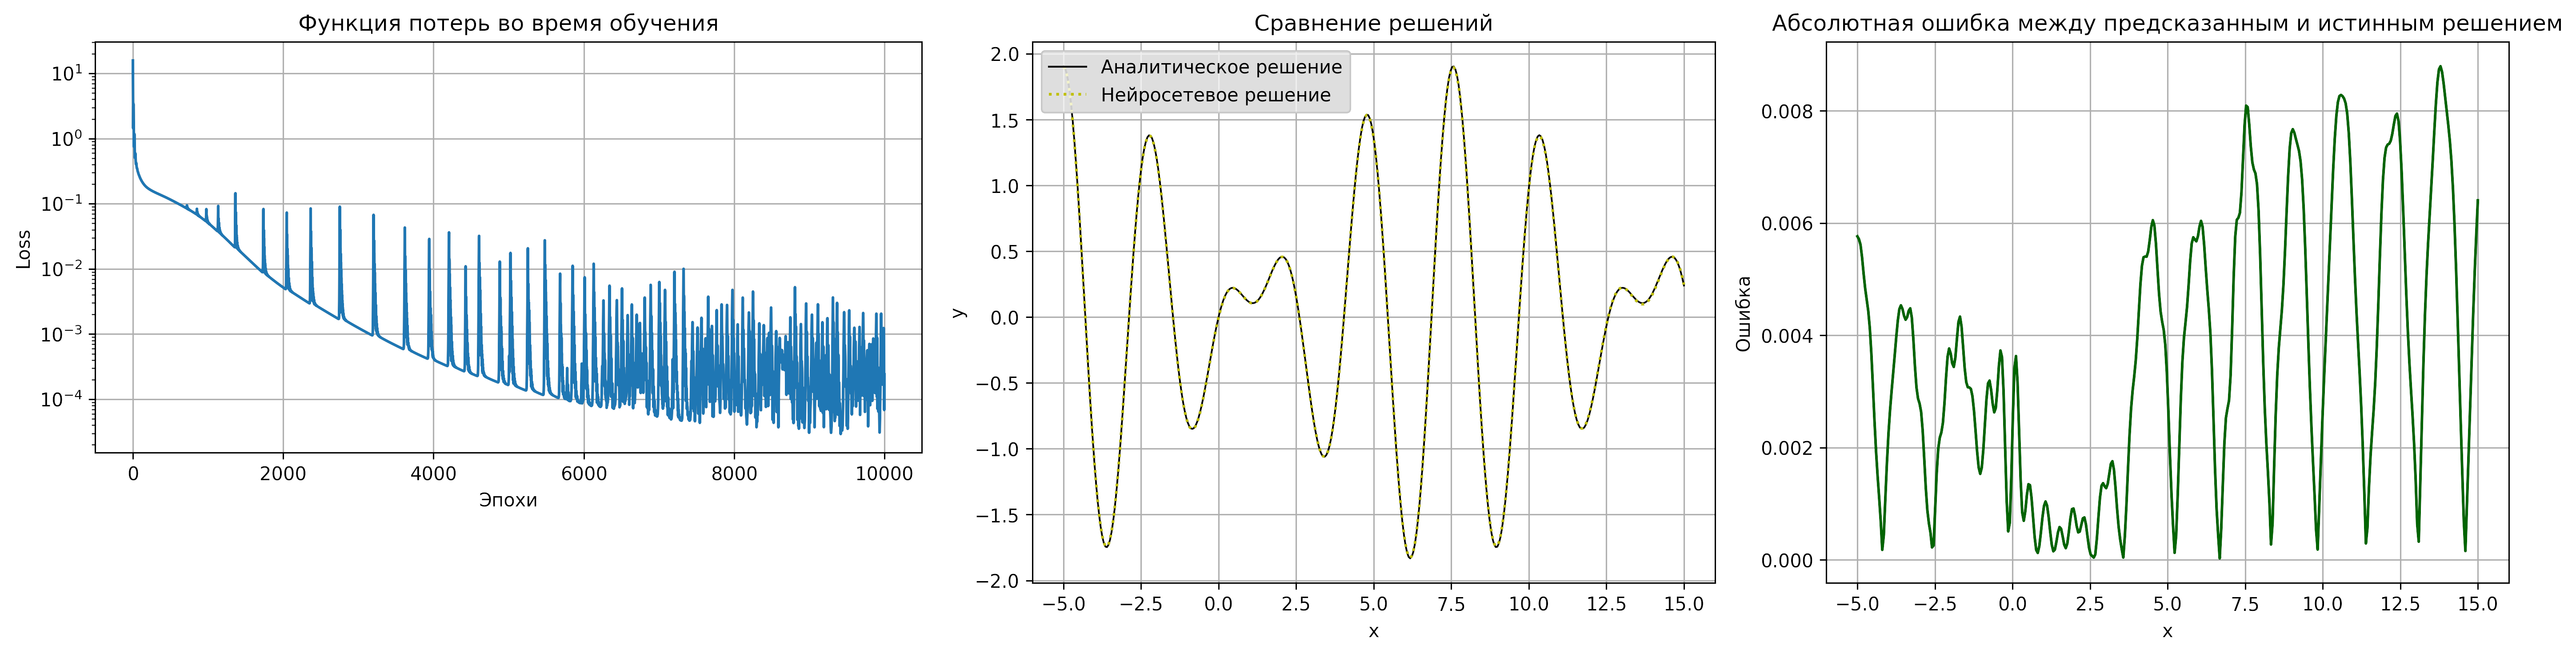
\includegraphics[width=1\textwidth]{images/Loss&x_alt_ODE.png}
        \caption{Функция потерь для альтернативной системы ОДУ}
        \label{fig:loss_alt}
    \end{figure}

    \begin{figure}[h!]
        \centering
        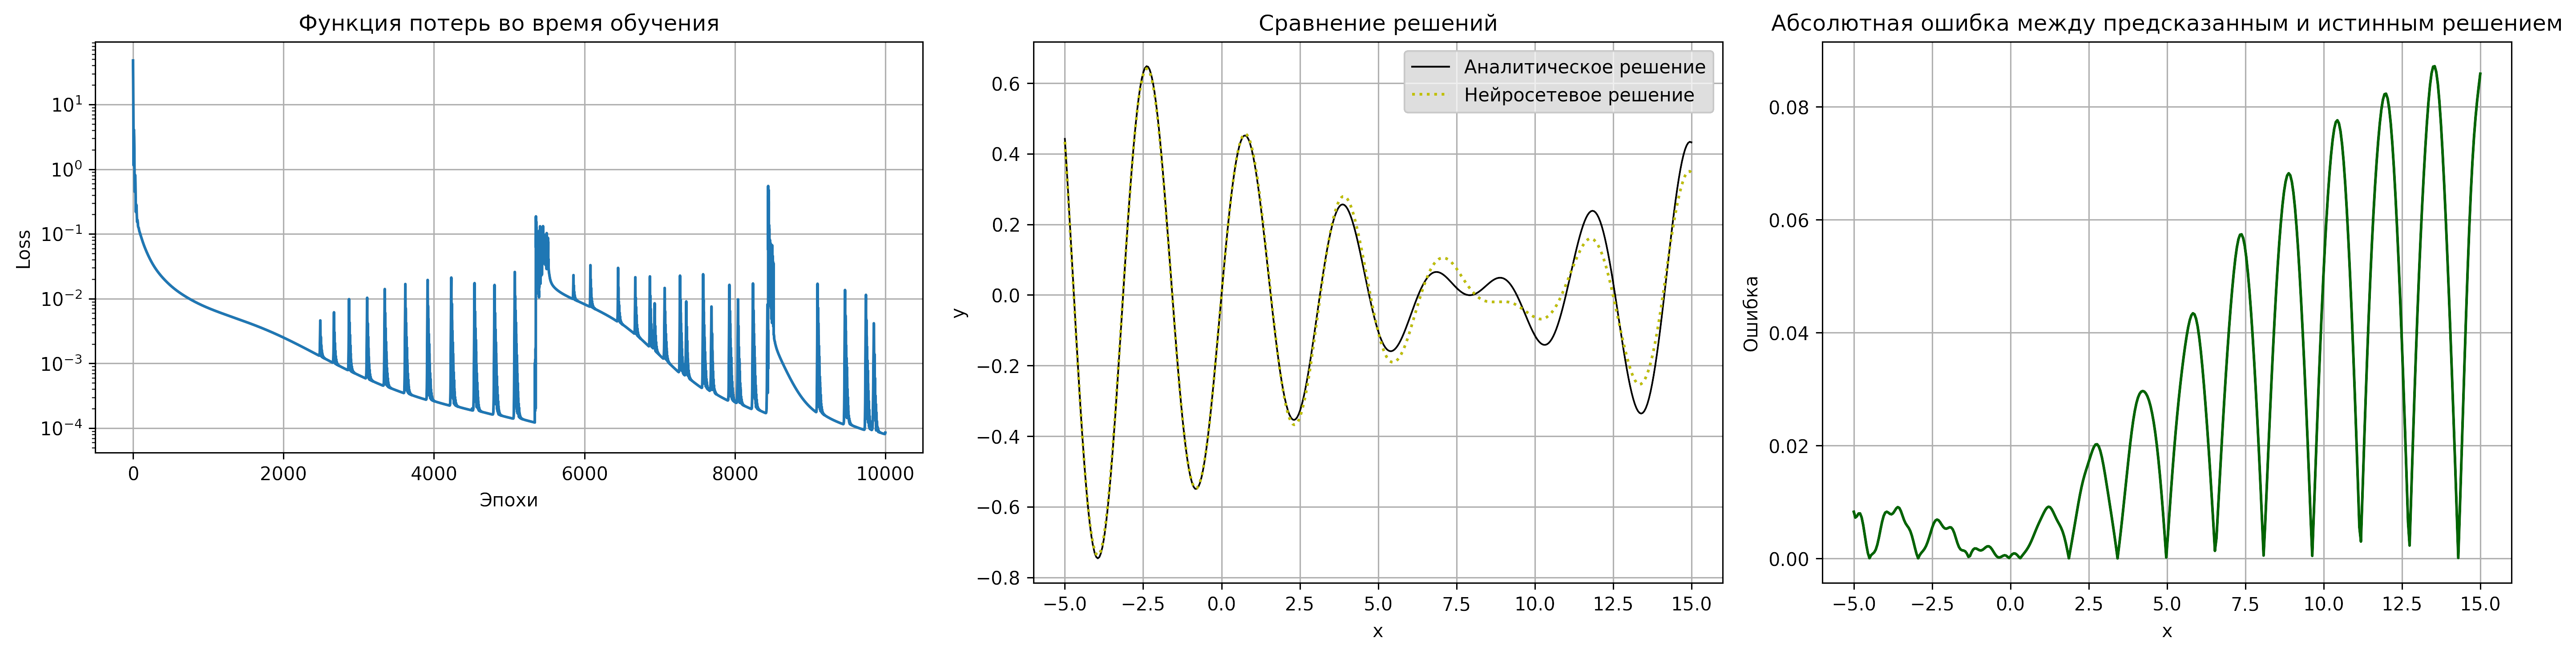
\includegraphics[width=1\textwidth]{images/Loss&x_alt_ODE_resonance.png}
        \caption{Функция потерь для альтернативной системы ОДУ с резонансом}
        \label{fig:loss_alt_resonance}
    \end{figure}

    \begin{table}[h!]
        \centering
        \begin{tabular}{|c|c|}
        \hline
        \textbf{MAE $x, 10^{-2}$} & \textbf{MAE $\dfrac{dx}{dt}, 10^{-2}$} \\
        \hline
        1,0991 & 2,3144 \\
        2,4914 & 5,1818 \\
        1,0468 & 2,2011 \\
        0,44066 & 0,96563 \\
        0,92337 & 1,9852 \\
        \hline
        \end{tabular}
        \caption{Альтернативная система ОДУ первого порядка без резонанся}
    \end{table}
        
\end{itemize}

\newpage
\section{Выводы}
Проведённое исследование показывает, что выбор постановки задачи Коши существенно влияет на эффективность и точность метода PINN.
Для конкретных приложений имеет смысл сравнить различные формулировки задачи, чтобы подобрать оптимальный вариант. В случае армонического осциллятора с вынуждающей силой.
\begin{itemize}
    \item Использование исходного уравнения второго порядка даёт быструю сходимость к точному решению, однако могут возникать проблемы с попаданием в локальные минимумы.
    \item Преобразование уравнения к системе первого порядка повышает устойчивость обучения, но может снижать точность и увеличивать время сходимости.
    \item Альтернативная система первого порядка позволяет достичь результата, близкого к исходному уравнению, при этом обладая более стабильным процессом оптимизации.
\end{itemize}
Полный код для воспроизведения результатов доступен в репозитории на GitHub:\\
\href{https://github.com/PracticalOscillations/Practice3}{https://github.com/PracticalOscillations/Practice3}.
Мы приглашаем заинтересованных исследователей использовать и развивать представленный подход.

\begin{thebibliography}{99}
\bibitem{Lagaris1998} Lagaris I.E., Likas A., Fotiadis D.I. Artificial neural networks for solving ordinary and partial differential equations. //IEEE Transactions on Neural Networks, 1998. T. 9. № 5. С. 987–1000.
\bibitem{Raissi2019} Raissi M., Perdikaris P., Karniadakis G.E. Physics-informed neural networks: A deep learning framework for solving forward and inverse problems involving nonlinear partial differential equations. //Journal of Computational Physics, 2019. T. 378. С. 686–707.
\bibitem{PyTorch} \href{https://pytorch.org/docs/stable/index.html}{PyTorch documentation}.
\end{thebibliography}

\end{document}
